%%
%% Copyright 2007, 2008, 2009 Elsevier Ltd
%%
%% This file is part of the 'Elsarticle Bundle'.
%% ---------------------------------------------
%%
%% It may be distributed under the conditions of the LaTeX Project Public
%% License, either version 1.2 of this license or (at your option) any
%% later version.  The latest version of this license is in
%%    http://www.latex-project.org/lppl.txt
%% and version 1.2 or later is part of all distributions of LaTeX
%% version 1999/12/01 or later.
%%
%% The list of all files belonging to the 'Elsarticle Bundle' is
%% given in the file `manifest.txt'.
%%

%% Template article for Elsevier's document class `elsarticle'
%% with numbered style bibliographic references
%% SP 2008/03/01

\documentclass[preprint,12pt, a4paper]{elsarticle}

%% Use the option review to obtain double line spacing
%% \documentclass[authoryear,preprint,review,12pt]{elsarticle}

%% For including figures, graphicx.sty has been loaded in
%% elsarticle.cls. If you prefer to use the old commands
%% please give \usepackage{epsfig}

%% The amssymb package provides various useful mathematical symbols
\usepackage{amssymb}
%% The amsthm package provides extended theorem environments
%% \usepackage{amsthm}

%% The lineno packages adds line numbers. Start line numbering with
%% \begin{linenumbers}, end it with \end{linenumbers}. Or switch it on
%% for the whole article with \linenumbers.
\usepackage{lineno}

\usepackage{float}
\restylefloat{table}

% ======== additional package not in SoftwareX template ========
\usepackage[colorlinks=true, urlcolor=blue, pdfborder={0 0 0}]{hyperref}
\usepackage{breakurl}
\usepackage[htt]{hyphenat}
%\usepackage{listings}
%\usepackage{xcolor}
%\usepackage{todonotes}

% \let\oldtodo\todo
% \renewcommand{\todo}[1]{\oldtodo[tickmarkheight=0.5em]{#1}}

\newcommand{\comment}[1]{}
% =================================================

\journal{SoftwareX}

\begin{document}
\begin{frontmatter}

\title{\texttt{davos}: a Python package ``smuggler'' for constructing
  lightweight reproducible notebooks}
\author{Paxton C. Fitzpatrick}
\author{Jeremy R. Manning\corref{cor}}
\ead{Jeremy.R.Manning@Dartmouth.edu}
\cortext[cor]{Corresponding author}
\address{Department of Psychological and Brain Sciences\\Dartmouth College, Hanover, NH 03755}

% ------------------------------------------------------ ABSTRACT ------------------------------------------------------

\begin{abstract}
% 100-word limit (though many published articles don't seem to conform
% to this?)

A core requirement of modern scientific research is replicability.
For computational research, replicability means that code should
produce the same results, even when run on different systems.  The
standard solution to improving replicability entails packaging a
project's dependencies along with its primary code base.  Existing
solutions vary in how deeply these dependencies are specified, ranging
from virtual environments (which specify all Python package versions),
to containers (which also specify the operating system), to
virtual machines (which also specify hardware layers of the system).
Each of these existing solutions requires installing or setting up a
system for running the desired code that must be packaged alongside
the primary code base.  Here we propose an even lighter-weight
solution than virtual environments: the \texttt{davos} library.  When
used in combination with a notebook-based Python project, \texttt{davos}
library provides a mechanism for specifying (and automatically
installing) the correct package versions of the project's.  This
enables researchers to share a complete reproducible environment using
a single iPython notebook file.

\end{abstract}


\begin{keyword}
Reproducibility \sep Open science \sep Python \sep Jupyter Notebook \sep Google Colaboratory \sep Package management
\end{keyword}

\end{frontmatter}


% ------------------------------------------------------ METADATA ------------------------------------------------------
\section*{Required Metadata}

\section*{Current code version}


\begin{table}[H]
\begin{tabular}{|l|p{6.5cm}|p{6.5cm}|}
\hline
\textbf{Nr.} & \textbf{Code metadata description} & \textbf{Notes} \\
\hline
C1 & Current code version &  v0.1.1 \\
\hline
C2 & Permanent link to code/repository used for this code version & \url{https://github.com/ContextLab/davos/tree/v0.1.1} \\
\hline
C3 & Code Ocean compute capsule & \\
\hline
C4 & Legal Code License & MIT \\
\hline
C5 & Code versioning system used & git \\
\hline
C6 & Software code languages, tools, and services used & Python, JavaScript, PyPI/pip, IPython, Jupyter, Ipykernel, PyZMQ. Additional tools used for tests: pytest, Selenium, Requests, mypy, GitHub Actions \\
\hline
C7 & Compilation requirements, operating environments \& dependencies & Dependencies:~Python$>$=3.6, packaging, setuptools.~Supported OSes: MacOS, Linux, Unix-like.~Supported IPython environments: Jupyter notebooks, JupyterLab, Google Colaboratory, Binder, IDE-based notebook editors. \\
\hline
C8 & Link to developer documentation/manual & \url{https://github.com/ContextLab/davos\#readme} \\
\hline
C9 & Support email for questions & contextualdynamics@gmail.com \\
\hline
\end{tabular}
\caption{Code metadata}
\label{}
\end{table}

\linenumbers


% --------------------------------------------- MOTIVATION & SIGNIFICANCE ----------------------------------------------
\section{Motivation and significance}

Jupyter (iPython) notebooks~\citep{KluyEtal16} have revolutionized
code sharing by providing a single filetype that combines text, code,
and figures.  For projects that depend on other software packages,
however, additional work is often required to enable the code to run
as its authors intended.  For example, a piece of software that
depends on version 0.8 of package \textit{X} may behave differently
(or may fail to run at all) if the user instead attempts to run the
code in an environment with version 0.9 of package \textit{X}.

% STOPPED HERE...



Sharing a project's code base is most valuable when that code may be
run on 



Modern scientific research frequently entails writing software code
for a wide variety of purposes throughout the scientific process.
Researchers across disciplines may design and implement complex
experiments; collect, store, and analyze large datasets; create
visualizations for presentations and publications; and share their
findings and techniques with peers, students, and the broader public
through tutorials, demos, workshops, and classes.  However, one
fundamental requirement of virtually any form of research-related code
is that its behavior and outputs remain consistent and predictable, no
matter when, where, or by whom it is run.  This stability can be
crucial, for example, to ensuring that data are collected under the
same conditions (e.g., across recordings, subjects, or physical
locations)
%^ or locations, e.g., in different test rooms, on different machines, at different sites, etc.
over multiple months or years, and that they can be accessed,
processed, and analyzed consistently by a research team that may be
spread across multiple institutions or countries.  Additionally,
modern open science practices encourage publicly sharing research code
and data so that others may explore, reproduce, learn from, and build
upon existing work.  Much of the benefit afforded by freely available
research code depends on users' ability to execute it and achieve the
same result as its original author.

Python \cite{vanR95} has become one of the most widely used and
fastest-growing scientific programming languages, in part by combining
an accessible, high-level syntax with a rich ecosystem of powerful
third-party tools that facilitate rapid development and collaboration
\cite{MullEtal15}.  The Python ecosystem offers an extensive data
science toolkit with platforms for interactive programming (e.g.,
Project Jupyter \cite{KluyEtal16}, Google Colaboratory),
community-maintained libraries for data manipulation (e.g., NumPy
\cite{HarrEtal20}, SciPy \cite{VirtEtal20}, Pandas \cite{McKi10}) and
visualization (e.g., Matplotlib \cite{Hunt07}, seaborn \cite{Wask21}),
frameworks for training complex machine learning models (e.g.,
scikit-learn \cite{PedrEtal11}, TensorFlow \cite{AbadEtal15}, Hugging
Face \cite{WolfEtal20}), and myriad other resources.  However, this
heavy emphasis on third-party libraries also presents a challenge to
writing and sharing stable, reproducible scientific Python code:
different versions of the same library may behave differently, adopt
changes in syntax, expose different functions and interfaces, add or
drop support for specific hardware or software, write (or expect to
read) files in different formats, fix (or introduce) bugs, and so on.
While these issues exist to some extent in any software language or
ecosystem, they have a particular impact on the Python community due
to its unusually rapid growth relative to other languages.  Ensuring
Python code behaves consistently over time and across users therefore
typically requires ensuring it is always run with the same specific
set of versions for each third-party package used.
%Ensuring Python code behaves consistently over time and across users therefore typically requires guaranteeing that the same specific version of each required third-party package is used, every time it is run.

One common approach to solving this problem is to create containerized
or virtualized Python environments (e.g., using Docker \cite{Merk14},
Singularity \cite{KurtEtal17}, or conda \cite{Anac12}) tailored to
individual applications.  A researcher may build such an environment
around a particular experiment or analysis pipeline, and exclusively
run their code from inside it, ``entering" and ``exiting" the
environment before and after each time they do so.  They can also
distribute their custom environment alongside their code as a
configuration file that explicitly lists required package versions,
enabling others to build identical copies for themselves.  This allows
research teams to deploy experiments on multiple machines for more
efficient data collection, collaborate on analyses without introducing
conflicts or inconsistencies, and publicly share their study designs
and results for others to reproduce, replicate, or adapt to study new
questions in the future.

While often effective, this approach bears two notable drawbacks.
First, it can add substantially to the technical knowledge, computing
resources, and initial setup needed to run or share the actual code of
interest.  For example, sharing code for an analysis or tutorial that
relies on a particular Docker image to run properly would of course
necessitate writing and distributing extra configuration files and
setup instructions.  But far more burdensomely, it also requires that
anyone who may want to run the code (in addition to the author seeking
to share it!) first be able to install and navigate additional
software that is likely far more complex and resource-intensive than
the actual analysis or tutorial code it facilitates running.  This can
introduce a need for both a degree of computer literacy and
computational resources that may not be universally accessible,
particularly to students or other early-career scientists hoping to
learn from publicly available tutorials.  These added prerequisites
clash with the simplicity and accessibility that have contributed to
Python's popularity, and can create significant barriers to both
contributing to and taking advantage of open science resources.

Second, while many existing tools allow users to initially populate a
Python environment with a fixed set of packages and package versions
(e.g., from a \texttt{requirements.txt}, \texttt{pyproject.toml},
\texttt{environment.yml}, \texttt{Pipfile}, \texttt{Dockerfile RUN}
instruction, etc.), few, if any, ensure that these specified
requirements \textit{remain} satisfied after they are first installed.
The ability to modify an environment after its creation is useful in
many cases (e.g., to install additional software, when
needed). However, this also makes it easy to inadvertently alter
existing packages, potentially leading to subtle issues with code that
relies on them.  For instance, suppose a researcher has implemented a
series of analyses using version 1.0 of ``Package \textit{X}," and
decides to perform an additional analysis that requires installing
``Package \textit{Y}."  If Package \textit{Y} depends on version 0.9
of Package \textit{X}, then Package \textit{X} will be downgraded to
accommodate this new requirement, potentially altering or breaking
previous analyses when they are rerun later, either by the researcher
or someone with whom they've shared their code.  Further, if some
analyses require Package \textit{Y} while others rely on features of
Package \textit{X} not implemented until version 1.0, it's unclear
which version the researcher should install in their environment.

%The \texttt{davos} package provides a novel, Python-native framework for creating, sharing, and running reproducible workflows that was designed to address each of these issues.
The \texttt{davos} package provides a novel, Python-native framework
for creating reproducible workflows that was designed to address each
of these issues. \texttt{davos} allows users to specify dependencies
directly within the code that...

\comment {
POINTS TO MAKE/THINGS TO SAY HERE TO WRAP UP (or maybe save some for impact section?):
- davos simplifies the process of writing, sharing, and running reproducible code (eliminates need for additional complex env management tools, syntax is simple, packages are just installed at runtime without additional setup beforehand, etc.)...
- ...it also provides stability/additional protections against accidental changes in ways other tools don't (i.e., addresses issue 2 above) by verifying (and installing if necessary) requirements each time code is run
- ... while simultaneously enabling new package management patterns (using multiple versions versions of package in same notebook, etc.)
- it's lightweight and intuitive (unlike big/complex env management tools like docker, etc.)
- "davos was specifically designed for use with Jupyter notebook environments, and can be used either on its own or in tandem with another environment management tool"
- "\texttt{davos} was designed specifically for use in Jupyter notebook (formerly called IPython notebook \cite{PereGran07}) environments, and supports Jupyter notebooks \cite{KluyEtal16}, JupyterLab \cite{GranGrou16}, Google Colaboratory, Binder \cite{RagaWill18}, and IDE-based notebook editors."

- maybe don't mention smuggle statement \& onion comment explicitly in this paragraph since they haven't been defined/explained yet, or if we do, then add some sort of "see \_\_\_ below" with \\ref to relevant subsection
}


%Introduce the scientific background and the motivation for developing the software.

%Explain why the software is important, and describe the exact (scientific) problem(s) it solves.

%Indicate in what way the software has contributed (or how it will contribute in the future) to the process of scientific discovery; if available, this is to be supported by citing a research paper using the software.

%Provide a description of the experimental setting (how does the user use the software?).

%Introduce related work in literature (cite or list algorithms used, other software etc.).


% ------------------------------------------------ SOFTWARE DESCRIPTION ------------------------------------------------
\section{Software description}
% Describe the software in as much as is necessary to establish a vocabulary needed to explain its impact.


\subsection{Software architecture}
The \texttt{davos} package is structured as two subpackages: a set of ``core" modules that implement...

% Give a short overview of the overall software architecture; provide a pictorial component overview or similar (if possible). If necessary provide implementation details.


\subsection{Software functionalities}%\label{sec:functionalities}

\subsubsection{The \texttt{smuggle} statement}
Importing \texttt{davos}\comment{in a Jupyter notebook} enables an additional Python keyword: ``\texttt{smuggle}".
The \texttt{smuggle} statement can be used as a drop-in replacement for Python's built-in \texttt{import} statement to load libraries, modules, and other objects into the current namespace.
However, whereas \texttt{import} will fail if the requested package is not installed locally, \texttt{smuggle} statements can handle missing packages on the fly.
If a smuggled package does not exist in the local environment, \texttt{davos} will install it, expose its contents to Python's \texttt{import} machinery, and load it into the namespace for immediate use.


\subsubsection{The onion comment}
For greater control over the behavior of \texttt{smuggle} statements, \texttt{davos} defines an additional construct called the \textit{onion comment}. An onion comment is a special type of inline comment that may be placed on a line containing a \texttt{smuggle} statement to customize how \texttt{davos} searches for the smuggled package locally and, if necessary, how it should be installed. Onion comments follow a simple syntax based on the ``type comment" syntax introduced in PEP 484 \cite{vanREtal14} and are designed to make managing packages via \texttt{davos} intuitive and familiar. To construct an onion comment, simply provide the name of the installer program (e.g., \texttt{pip}) and the same arguments one would use to install the package as desired manually via the command line (see Fig.~\ref{fig:snippet1}).

\begin{figure}[h]
\centering
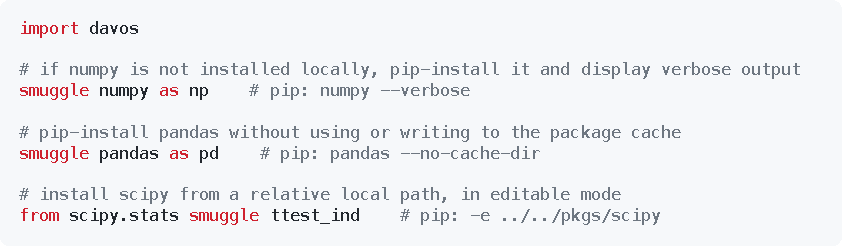
\includegraphics[width=\textwidth]{snippets/snippet1.pdf}
\caption{\small \textbf{Figure 1}}
\label{fig:snippet1}
\end{figure}



%\definecolor{backgroundgrey}{RGB}{244,246,249}
%\definecolor{commentgrey}{RGB}{91,99,110}
%\definecolor{keywordred}{RGB}{194,11,36}
%
%\lstset{
%    backgroundcolor=\color{backgroundgrey},
%    basicstyle=\footnotesize\fontfamily{qag}\selectfont, %\ttfamily,
%    breaklines=true,
%    commentstyle=\color{commentgrey},
%    language=Python,
%    emph={import, smuggle, from, as},
%    emphstyle=\color{keywordred},
%}
%
%\begin{lstlisting}
%import davos
%
%# if numpy is not installed locally, pip-install it and display verbose output
%smuggle numpy as np    # pip: numpy --verbose
%
%# pip-install pandas without using or writing to the package cache
%smuggle pandas as pd    # pip: pandas --no-cache-dir
%
%# install scipy from a relative local path, in editable mode
%from scipy.stats smuggle ttest_ind # pip: -e ../../pkgs/scipy
%\end{lstlisting}

\subsubsection{The \texttt{davos} config}

\subsubsection{Additional functionality}

% Present the major functionalities of the software.


\subsection{Sample code snippets analysis (optional)}


% ----------------------------------------------- ILLUSTRATIVE EXAMPLES ------------------------------------------------
\section{Illustrative Examples}
% Provide at least one illustrative example to demonstrate the major functions.

% Optional: you may include one explanatory video that will appear next to your article, in the right hand side panel. (Please upload any video as a single supplementary file with your article. Only one MP4 formatted, with 50MB maximum size, video is possible per article. Recommended video dimensions are 640 x 480 at a maximum of 30 frames/second. Prior to submission please test and validate your .mp4 file at $ http://elsevier-apps.sciverse.com/GadgetVideoPodcastPlayerWeb/verification$. This tool will display your video exactly in the same way as it will appear on ScienceDirect.).


% ------------------------------------------------------- IMPACT -------------------------------------------------------
\section{Impact}
\comment{
- emphasize research domain-independent application (Journal's goals/values page says they prioritize this in submissions)
- applicability not limited to research
    - regression (?) testing
    - ***^^not sure this should be included -- hurts framing of davos as "research software"***
- makes writing and running publicly available reproducible code more accessible (lowers required software comfort/familiarity level \& computing resources vs. installing docker/singularity/conda)
    - also removes these requirements from other scenarios, e.g., easier for new/less experienced students/RAs to get involved with analyses
- mention something about not having to teach environment management to teach day 1 python lesson, or spend hours debugging conda installation in order to share tutorial or demo with students
    - e.g., "researchers who teach \_\_\_ may be familiar with the experience of running a lesson or workshop that requires students to use Docker (or similar...) to run their code, only to spend the majority of class time debugging students' computing environments rather than teaching the lesson itself."
}

Since its initial release, \texttt{davos} has found use in a variety
of applications.  In addition to managing data analysis environments
for multiple ongoing research studies, \texttt{davos} is being used by
both students and instructors in programming courses such as
\href{https://github.com/ContextLab/storytelling-with-data}{\textit{Storytelling
    with Data}} \cite{Mann21b} (an open course on data science,
visualization, and communication) to simplify distributing lessons and
submitting assignments, as well as in online demos such as
{\texttt{abstract2paper}} \cite{Mann21a} (an example application of
\href{https://github.com/EleutherAI/gpt-neo}{GPT-Neo}) to share
ready-to-run code that installs dependencies automatically.

%\textbf{This is the main section of the article and the reviewers weight the description here appropriately}

%Indicate in what way new research questions can be pursued as a result of the software (if any).

%Indicate in what way, and to what extent, the pursuit of existing research questions is improved (if so).

%Indicate in what way the software has changed the daily practice of its users (if so).

%Indicate how widespread the use of the software is within and outside the intended user group.

%Indicate in what way the software is used in commercial settings and/or how it led to the creation of spin-off companies (if so).


% ---------------------------------------------------- CONCLUSIONS -----------------------------------------------------
\section{Conclusions}
% Set out the conclusion of this original software publication.


\section*{Author Contributions}
\textbf{Paxton C. Fitzpatrick}: Conceptualization, Methodology, Software, Validation, Writing - Original Draft, Visualization. \textbf{Jeremy R. Manning}: Conceptualization, Resources, Writing - Review \& Editing, Supervision, Funding acquisition.

\section*{Funding}
Our work was supported in part by NSF grant number 2145172 to J.R.M.
The content is solely the responsibility of the authors and does not necessarily represent the official views of our supporting organizations.


\section*{Declaration of Competing Interest}
We wish to confirm that there are no known conflicts of interest associated with this publication and there has been no significant financial support for this work that could have influenced its outcome.


\section*{Acknowledgements}


%---------------------------------------------------- BIBLIOGRAPHY -----------------------------------------------------
\bibliographystyle{elsarticle-num}
\bibliography{main.bib}

\end{document}

